\documentclass[tikz]{standalone}
%\documentclass{article}
\usepackage{graphicx}
\usetikzlibrary{calc}

\begin{document}
  \begin{figure}[htb]
    \centering
    
    \begin{minipage}{0.48\textwidth}

      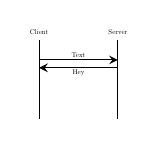
\begin{tikzpicture}
        \coordinate (a) at (0,0);
        \coordinate (b) at (0,1);
        \coordinate (c) at (1,0);
        \coordinate (d) at (1,1);
        \draw (a) -- (b)node[pos=1.1,scale=0.25]{Client} (c) -- (d)node[pos=1.1,scale=0.25]{Server};
        \draw[-stealth] ($(a)!0.75!(b)$) -- node[above,scale=0.25,midway]{Text}($(c)!0.75!(d)$);
        \draw[stealth-] ($(a)!0.65!(b)$) -- node[below,scale=0.25,midway]{Hey} ($(c)!0.65!(d)$);
      \end{tikzpicture}

      %\includegraphics[width=\linewidth]{example-image}
      %\caption{Some picture}
    \end{minipage}
    %\hfill
    %\medskip
  \end{figure}
\end{document}
